\section{Botnets}
\label{sec:botnets}

A \textit{botnet} is a network made up of unaware remote-controlled computers, typically used for malicious purposes.
A \textit{bot} is the malware that makes the infected host remotely controllable by a server — namely a \textit{controller} — instructed by an attacker. Once started, the bot contacts the controller to join the \textit{botnet} and polls it for commands to execute.

Some botnets consist of hundreds of thousands — or even millions — of computers. Since they allow such a lot of different computers to act in unison, a botnet could be used to perform \textit{distributed DDoS attacks}, \textit{massive spam campaign}, \textit{click frauds}, \textit{Bitcoin mining}, or used to \textit{distribute other malwares} — e.g. keyloggers and crypto lockers \cite{anderson2008security}. \ref{fig:botnet-showcase} depicts a simple but common botnet-based application. From this brief description about botnets it is possible to guess their economic implications.

\begin{figure}[tp]
  \centering
  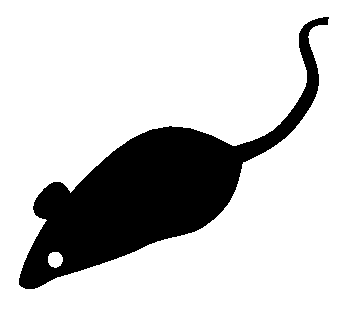
\includegraphics{./fig/acmlarge-mouse}
  \caption{A botnet showcase. (1) The attacker spreads bots via an infection vector — e.g. a trojan horse. (2) The infected hosts join the botnet, being remotely controllable by the attacker, via a command\&control server. (3) The computational power of the botnet is rent, for wichever malicious purpose, making the attacker gaining a lot of profits. (4) The attacker instructs the botnet to perform a spamming campaign, as requested by its client.}
    \label{fig:botnet-showcase}
\end{figure}

The \textit{command and control (C\&C)} is the component responsible for the distribution of commands to bots. Botnets can be controlled in several different ways, depending on how C\&C is implemented. In its simplest form, the C\&C implements a \textit{centralized client-server architecture} (i.e. \textit{C\&C server}), where bots poll a web server for commands to execute. Such a botnet is easy to stop — monitor what web servers a bot is connecting to, then take them down and causing the bots to be unable to communicate with the attacker. In a more advanced form, it implements a \textit{peer-to-peer (P2P) architecture} (i.e. \textit{C\&C node}), where bots instruct (are instructed by) other nearby bots, thus providing the botnet with a high degree of availability and redundancy. Since no single point of control can be identified, such botnets cannot be neutered only by disabling specific nodes. Therefore, defensive strategies are based on issuing fake commands or by isolating the bots from each other. Things are made harder since botnets started communicating, not only through encrypted channels, but via anonimous networks — such as Tor — where it’s theoretically impossible to figure out the botnet topology.

The \textit{ZeroAccess botnet} is an important example. The ZeroAccess botnet is one of the largest known botnets with a population upwards of 1.9 million computers, generating profits through Bitcoin mining and click frauds \cite{zeroaccess-symantec-blog,zeroaccess-symantec-definition}.
A key feature of the ZeroAccess botnet is its use of a P2P based C\&C, making it highly resistant to any take-down attempts.
